\documentclass[12pt,]{article}
\usepackage{lmodern}
\usepackage{amssymb,amsmath}
\usepackage{ifxetex,ifluatex}
\usepackage{fixltx2e} % provides \textsubscript
\ifnum 0\ifxetex 1\fi\ifluatex 1\fi=0 % if pdftex
  \usepackage[T1]{fontenc}
  \usepackage[utf8]{inputenc}
\else % if luatex or xelatex
  \ifxetex
    \usepackage{mathspec}
    \usepackage{xltxtra,xunicode}
  \else
    \usepackage{fontspec}
  \fi
  \defaultfontfeatures{Mapping=tex-text,Scale=MatchLowercase}
  \newcommand{\euro}{€}
\fi
% use upquote if available, for straight quotes in verbatim environments
\IfFileExists{upquote.sty}{\usepackage{upquote}}{}
% use microtype if available
\IfFileExists{microtype.sty}{%
\usepackage{microtype}
\UseMicrotypeSet[protrusion]{basicmath} % disable protrusion for tt fonts
}{}
\usepackage[margin=1in]{geometry}
\usepackage{graphicx}
\makeatletter
\def\maxwidth{\ifdim\Gin@nat@width>\linewidth\linewidth\else\Gin@nat@width\fi}
\def\maxheight{\ifdim\Gin@nat@height>\textheight\textheight\else\Gin@nat@height\fi}
\makeatother
% Scale images if necessary, so that they will not overflow the page
% margins by default, and it is still possible to overwrite the defaults
% using explicit options in \includegraphics[width, height, ...]{}
\setkeys{Gin}{width=\maxwidth,height=\maxheight,keepaspectratio}
\ifxetex
  \usepackage[setpagesize=false, % page size defined by xetex
              unicode=false, % unicode breaks when used with xetex
              xetex]{hyperref}
\else
  \usepackage[unicode=true]{hyperref}
\fi
\hypersetup{breaklinks=true,
            bookmarks=true,
            pdfauthor={},
            pdftitle={Is the Tea Party Libertarian, Authoritarian, or Something Else?},
            colorlinks=true,
            citecolor=black,
            urlcolor=red,
            linkcolor=black,
            pdfborder={0 0 0}}
\urlstyle{same}  % don't use monospace font for urls
\setlength{\parindent}{0pt}
\setlength{\parskip}{6pt plus 2pt minus 1pt}
\setlength{\emergencystretch}{3em}  % prevent overfull lines
\setcounter{secnumdepth}{0}

%%% Change title format to be more compact
\usepackage{titling}
\setlength{\droptitle}{-2em}
  \title{Supplementary Information for ``Is the Tea Party Libertarian, Authoritarian, or Something Else?''
\vspace{1.25em}}
  \pretitle{\vspace{\droptitle}\centering\huge}
  \posttitle{\par}
  \author{}
  \preauthor{}\postauthor{}
  \date{}
  \predate{}\postdate{}


\usepackage{setspace}


\begin{document}

\maketitle

\paragraph{Contents}\label{contents}

\begin{enumerate}
\def\labelenumi{\arabic{enumi}.}
\itemsep1pt\parskip0pt\parsep0pt
\item
Additional information on Factor Analysis
\item
  Scree plot for factor model
\item
  Numerical factor loadings
\item
  Including Party ID as a covariate
\item
  Estimated effects of misarchism on Party ID and Conservatism
\item
Bayesian Model Averaging
\item
Multiple Imputation
\item
Matching and Sensitivity
\item
References
\end{enumerate}

Additional information on Factor Analysis

We used an oblique rotation which allows for factors to be correlated. This is
  appropriate here because, while we argue that moral statism and
  anti-governmentalism are unique and distinct, they are likely to be
  correlated. We use maximum likelihood as the factoring method because
  it has a more formal statistical basis than other methods and is
  widely seen as one of the optimal methods. See Fabrigar et al. (1999). We estimate two factors, which a scree plot (below) suggests to be the optimal number.
  
  For \emph{N} equal to 5914, a chi-square test of the hypothesis that two factors is
  sufficient is equal to 900.727 with a p-value of 0, suggesting that
  two factors are not sufficient, as we would expect. That said, the
  root mean square of the residuals is 0.044 and the Tucker-Lewis Index
  for factor reliability score is 0.869, both of which are near the
  conventional cutoffs of .05 and .9, respectively.

\begin{figure}[htbp]
\centering
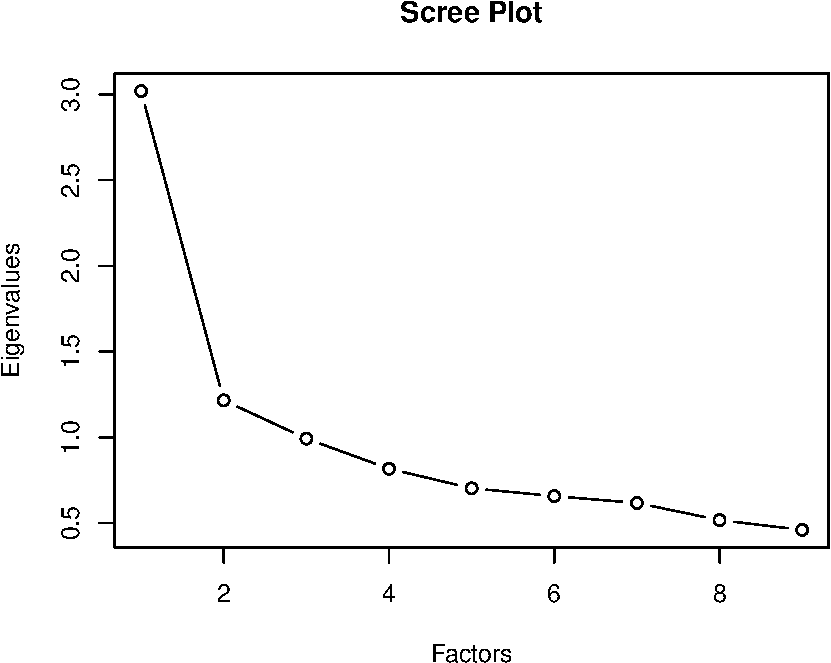
\includegraphics{figures/scree-1.pdf}
\caption{Scree plot shows elbow at two factors}
\end{figure}

\clearpage

\begin{table}[ht]
\centering
\begin{tabular}{rrr}
  \hline
 & ML1 & ML2 \\ 
  \hline
Family & 0.03 & 0.59 \\ 
  Guns & 0.40 & -0.05 \\ 
  Intolerant & -0.12 & 0.44 \\ 
  Morals & -0.22 & 0.36 \\ 
  Wiretapping & 0.21 & 0.35 \\ 
  Defense & 0.04 & 0.49 \\ 
  Services & 0.78 & 0.01 \\ 
  Immigration & -0.24 & 0.38 \\ 
  Jobs & 0.61 & -0.04 \\ 
   \hline
\end{tabular}
\caption{Factor Loadings} 
\label{Factor Loadings}
\end{table}

\begin{figure}[htbp]
\centering
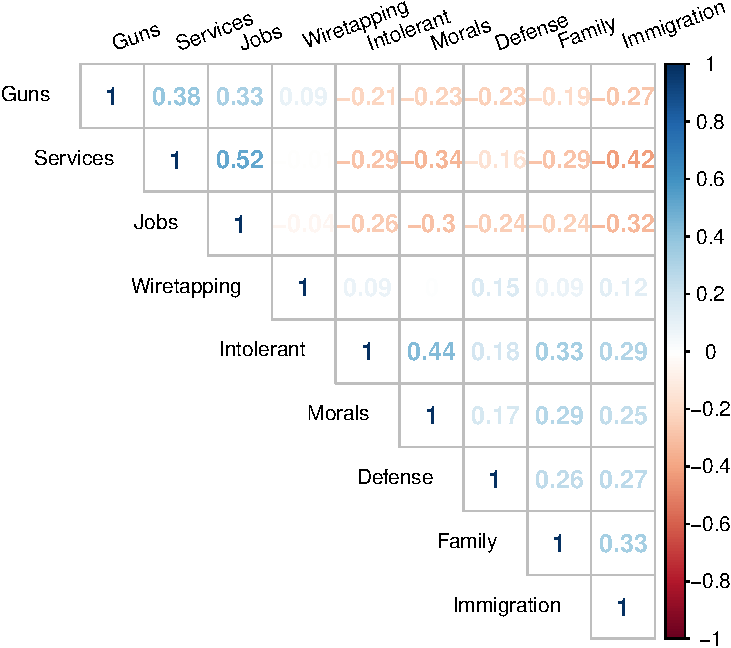
\includegraphics{figures/descriptives-1.pdf}
\caption{Correlation plot for different dimensions of right-wing
attitudes}
\end{figure}



\clearpage

\begin{table}[!htbp] \centering 
  \caption{Alternative Dependent Variables for Model 2} 
  \label{} 
\footnotesize 
\begin{tabular}{@{\extracolsep{5pt}}lcc} 
\\[-1.8ex]\hline 
\hline \\[-1.8ex] 
 & \multicolumn{2}{c}{\textit{Dependent variable:}} \\ 
\cline{2-3} 
\\[-1.8ex] & PartyID (Republican) & Conservatism \\ 
\\[-1.8ex] & (1) & (2)\\ 
\hline \\[-1.8ex] 
 Gender (Male) & $-$0.006 & 0.008 \\ 
  & (0.013) & (0.014) \\ 
  Income & 0.032$^{**}$ & $-$0.003 \\ 
  & (0.015) & (0.016) \\ 
  Age & $-$0.057$^{***}$ & 0.025 \\ 
  & (0.014) & (0.016) \\ 
  Race (White) & 0.076$^{***}$ & $-$0.058$^{***}$ \\ 
  & (0.015) & (0.017) \\ 
  Education & 0.044$^{***}$ & $-$0.024 \\ 
  & (0.015) & (0.017) \\ 
  Obama & $-$0.545$^{***}$ & $-$0.103$^{***}$ \\ 
  & (0.020) & (0.025) \\ 
  Authoritarianism & $-$0.029$^{**}$ & 0.039$^{**}$ \\ 
  & (0.015) & (0.016) \\ 
  BornAgain & 0.016 & 0.030$^{*}$ \\ 
  & (0.014) & (0.015) \\ 
  Religion & 0.001 & 0.038$^{**}$ \\ 
  & (0.015) & (0.017) \\ 
  PartyID (Republican) &  & 0.321$^{***}$ \\ 
  &  & (0.022) \\ 
  FoxNews & 0.039$^{**}$ & 0.059$^{***}$ \\ 
  & (0.015) & (0.017) \\ 
  Conservatism & 0.256$^{***}$ &  \\ 
  & (0.018) &  \\ 
  MoralStatism & $-$0.001 & 0.259$^{***}$ \\ 
  & (0.024) & (0.026) \\ 
  Government & $-$0.103$^{***}$ & $-$0.100$^{***}$ \\ 
  & (0.023) & (0.026) \\ 
  MoralStatism*Government & 0.025 & 0.044 \\ 
  & (0.026) & (0.029) \\ 
  Constant & $-$0.051$^{***}$ & $-$0.009 \\ 
  & (0.019) & (0.022) \\ 
 \hline \\[-1.8ex] 
Observations & 2,406 & 2,406 \\ 
R$^{2}$ & 0.674 & 0.523 \\ 
Adjusted R$^{2}$ & 0.673 & 0.521 \\ 
Residual Std. Error (df = 2391) & 0.305 & 0.342 \\ 
F Statistic (df = 14; 2391) & 354.000$^{***}$ & 187.000$^{***}$ \\ 
\hline 
\hline \\[-1.8ex] 
\textit{Note:}  & \multicolumn{2}{r}{$^{*}$p$<$0.1; $^{**}$p$<$0.05; $^{***}$p$<$0.01} \\ 
\end{tabular} 
\end{table}



\begin{table}[!htbp] \centering 
  \caption{Including ideology in factor model and removing from regression model} 
  \label{} 
\footnotesize 
\begin{tabular}{@{\extracolsep{5pt}}lc} 
\\[-1.8ex]\hline 
\hline \\[-1.8ex] 
 & \multicolumn{1}{c}{\textit{Dependent variable:}} \\ 
\cline{2-2} 
\\[-1.8ex] & Tea Party Support \\ 
\hline \\[-1.8ex] 
 Gender (Male) & 0.116 \\ 
  & (0.128) \\ 
  Income & $-$0.301$^{**}$ \\ 
  & (0.148) \\ 
  Age & $-$0.343$^{**}$ \\ 
  & (0.144) \\ 
  Race (White) & $-$0.404$^{**}$ \\ 
  & (0.169) \\ 
  Education & 0.066 \\ 
  & (0.158) \\ 
  Obama & $-$1.250$^{***}$ \\ 
  & (0.222) \\ 
  Authoritarianism & 0.035 \\ 
  & (0.148) \\ 
  BornAgain & 0.298$^{**}$ \\ 
  & (0.135) \\ 
  Religion & $-$0.013 \\ 
  & (0.155) \\ 
  PartyID (Republican) & 0.512$^{**}$ \\ 
  & (0.199) \\ 
  FoxNews & 0.707$^{***}$ \\ 
  & (0.133) \\ 
  MoralStatism & $-$0.556$^{**}$ \\ 
  & (0.261) \\ 
  Government & 0.923$^{***}$ \\ 
  & (0.276) \\ 
  MoralStatism*Government & 1.380$^{***}$ \\ 
  & (0.268) \\ 
  Constant & $-$2.700$^{***}$ \\ 
  & (0.214) \\ 
 \hline \\[-1.8ex] 
Observations & 2,406 \\ 
Log Likelihood & $-$830.000 \\ 
Akaike Inf. Crit. & 1,690.000 \\ 
\hline 
\hline \\[-1.8ex] 
\textit{Note:}  & \multicolumn{1}{r}{$^{*}$p$<$0.1; $^{**}$p$<$0.05; $^{***}$p$<$0.01} \\ 
\end{tabular} 
\end{table}

Individuals characterized by the highest observed levels of moral
statism also in the 90th percentile of anti-governmentalism (below a
value of -.7 on the governmentalism factor) have a probability of
supporting the Tea Party around 40\%. To be more precise, moving from
minimum to maxium moral statism while in the 10th percentile of
governmentalism increases the probability of supporting the Tea Party by
.39 (sd=.07) more than it would in the 90th percentile of
govermentalism, from .01 (sd=.00) to .42, (sd=.07) rather than .05
(sd=.02) to .03 (sd=.02).

\clearpage

\subsubsection{Bayesian Model Averaging}\label{bayesian-model-averaging}

regression results such as those presented above are sometimes sensitive
to minor differences in model specification, such as including or
excluding one variable. One risk is publication bias, if researchers
prefer models that confirm their hypotheses. Another is loss of
efficiency if too many unnecessary variables are included. Finally, an
\emph{ad hoc} approach leads to incomplete representations of model
uncertainty (J. M. Montgomery and Nyhan 2010, 4).

In particular, a version of the R package \emph{BMA} modified by
Mongtomery and Nyhan was used to search over the entire model space of
Model 2.\footnote{The analysis was conducted using the
  \emph{bic.glmMN()} function, which is a version of the
  \emph{bic.glm()} function in the R package \emph{BMA}. See (Raftery et
  al. 2015) and (J. M. Montgomery and Nyhan 2010)} The analysis uses
uniform priors for all independent variables and the only restriction is
that the interaction term and its two component variables are required
to enter or not enter models together.\footnote{Options were set to be
  least restrictive. No Occam's Window was used to narrow the models
  selected by the initial leap algorithm run over the entire model space
  and, following Montgomery and Nyhan (pp.~21), the number of best
  models of each size returned by the leaps algorithm was set to 100,000}
In the end, 4,096 models were selected.

The results show that the misarchist terms are highly robust to model
selection, with a posterior probability of inclusion equal to 100\% (one
minus the cumulative posterior probability of all models excluding
them). The expected value of the coefficient for \emph{MoralStatism} is
.78 (sd=.29), for \emph{Governmentalism} it is -.71 (sd=.26), and for
the interaction term it is -1.43 (sd=.31). \emph{Obama} and
\emph{FoxNews} also had probabilities of inclusion equal to 100\% with
expected values not dissimilar to those estimated in Model 2. \emph{Age}
and \emph{Race} had probabilities of inclusion greater than 50\% but
with unstable signs, as indicated by expected values hardly
distinguishable from zero. All other variables had probabilities of
inclusion less than 50\%. More detailed graphical information is
reported in Supplementary Information.

In the main models reported above, we have consciously chosen to include
a large number of control variables because we are presently most
concerned with testing our hypotheses and ruling out rival hypotheses.
BMA provides further evidence that the models presented above likely
contain superfluous independent variables. Though we believe it is best
to rely primarily on the conservative estimates reported above, we
briefly report how our coefficients of interest would change under
different specifications suggested by the BMA. In a model with just
those variables found to be the most robust to model selection
(\emph{Fox News}, \emph{Obama}, \emph{MoralStatism}, and
\emph{Governmentalism}), moving from 10th percentile of
\emph{MoralStatism} to 90th within the 90th of \emph{Governmentalism},
is associated with the probablitity of supporting the Tea Party
increasing from .01 (sd=.00) to .50 (sd=.06). Thus, the results from
Bayesian Model Averaging suggest the main results reported above are
highly robust and, if anything, conservative estimates of the partial
correlation between misarchism and Tea Party support.

\begin{figure}[htbp]
\centering
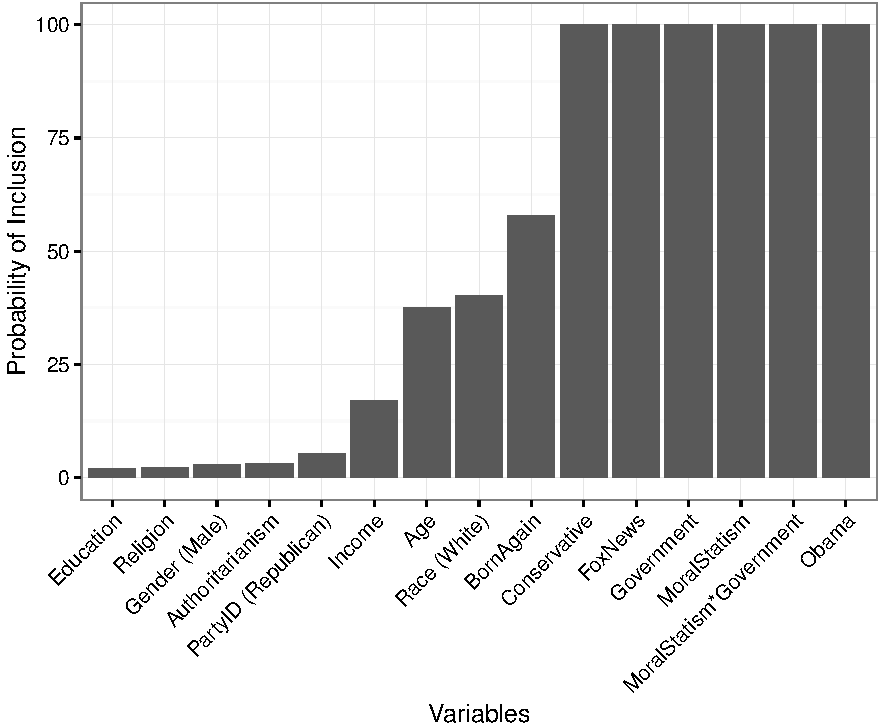
\includegraphics{figures/bma2-1.pdf}
\caption{Inclusion Probabilites from Bayesian Model Averaging}
\end{figure}

\clearpage

\begin{figure}[htbp]
\centering
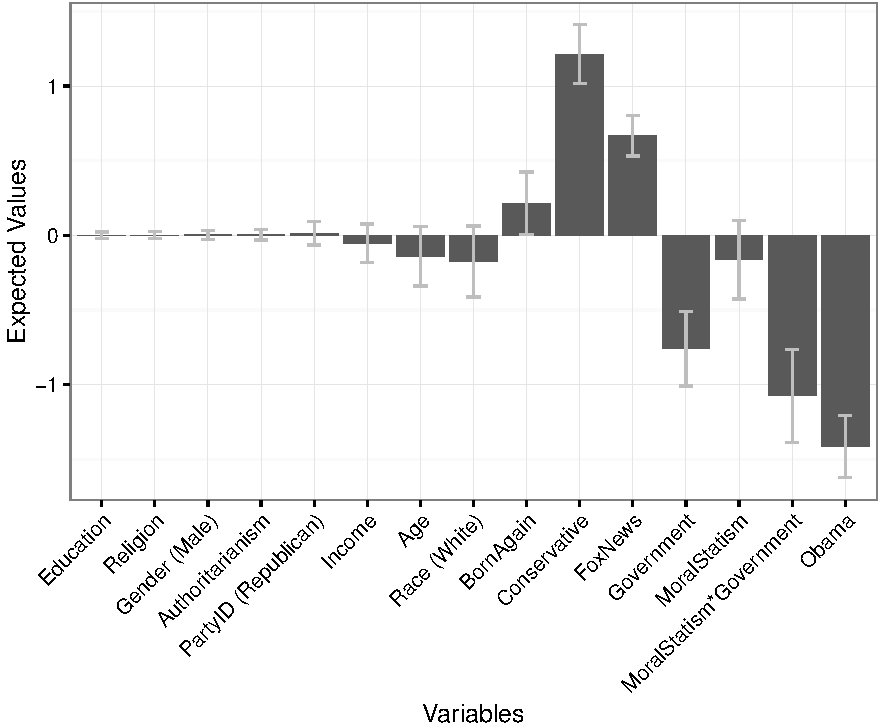
\includegraphics{figures/bma3-1.pdf}
\caption{Expected Values from Bayesian Model Averaging}
\end{figure}

\clearpage

\subsubsection{Multiple Imputation}\label{multiple-imputation}

In particular, if relative misarchists were more (or less) likely to
respond to certain questions than other respondents, we may have
over-estimated (or under-estimated) the true partial correlation between
our misarchist terms and Tea Party support. Multiple imputation refers
to the process of using the information from observed variables to infer
the most likely values for all missing cells. The process finishes by
producing a set of new datasets each of which samples from the
predictive distribution to assign most likely values to each missing
cell. After multiple imputation, the models discussed above are
re-estimated on each imputed dataset and the results are combined using
``Rubin's rules.'' Specifically, we use the R package \emph{Amelia}
(Honaker, King, and Blackwell 2008) to generate 10 versions of the ANES
dataset with missing values imputed and \emph{Zelig} (Imai, King, and Lau 2009) to obtain pooled
regression results. The multiple imputation algorithm only assumes that
missing values are ``missing at random,'' not necessarily ``missing
completely at random.'' In this context, ``missing at random'' only
means that missingness is dependent on the observed variables.

After pooling the results, the estimates remain substantially the same.
\emph{MoralStatism}, \emph{Governmentalism}, and the interaction term
remain signed as in Model 2 with high statistical significance (.98,
p\textless{}.00; -.68, p\textless{}.00; -1.35, p\textless{}.00,
respectively). \emph{FoxNews} and \emph{BornAgain} also remain
substantially the same. Graphical diagnostics for overimputation,
dispersion, and comparing pre- and post-imputation densities for our
main variables suggest no problems or anomolies in the imputation
procedures. \clearpage

\begin{table}[ht]
\centering
\begin{tabular}{rrrrr}
  \hline
 & Value & Std. Error & t-stat & p-value \\ 
  \hline
(Intercept) & -2.07 & 0.11 & -18.21 & 0.00 \\ 
  Gender (Female) & -0.10 & 0.09 & -1.21 & 0.23 \\ 
  Income & -0.27 & 0.11 & -2.54 & 0.01 \\ 
  Age & -0.22 & 0.10 & -2.27 & 0.02 \\ 
  Race (White) & -0.29 & 0.11 & -2.77 & 0.01 \\ 
  Education & -0.02 & 0.11 & -0.21 & 0.83 \\ 
  Obama & -0.95 & 0.14 & -6.92 & 0.00 \\ 
  Authoritarianism & 0.10 & 0.10 & 0.97 & 0.33 \\ 
  BornAgain & -0.26 & 0.09 & -2.76 & 0.01 \\ 
  Religion & 0.03 & 0.10 & 0.32 & 0.75 \\ 
  PartyID (Republican) & 0.21 & 0.13 & 1.61 & 0.11 \\ 
  FoxNews & 0.71 & 0.10 & 7.40 & 0.00 \\ 
  Conservatism & 0.98 & 0.13 & 7.46 & 0.00 \\ 
  MoralStatism & 0.07 & 0.20 & 0.35 & 0.73 \\ 
  Governmentalism & -0.86 & 0.18 & -4.70 & 0.00 \\ 
  MoralStatism*Governmentalism & -0.85 & 0.21 & -3.96 & 0.00 \\ 
   \hline
\end{tabular}
\caption{Pooled Logistic Regression Results From 10 Multiple Imputations} 
\end{table}

\clearpage

\begin{figure}[htbp]
\centering
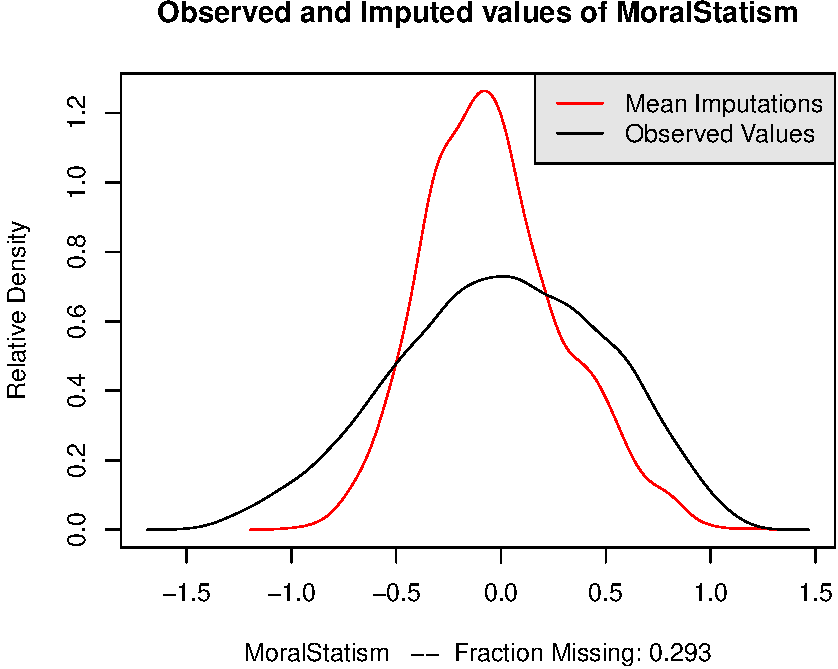
\includegraphics{figures/missing2-1.pdf}
\caption{Distributions Before and After Multiple Imputation (1)}
\end{figure}

\begin{figure}[htbp]
\centering
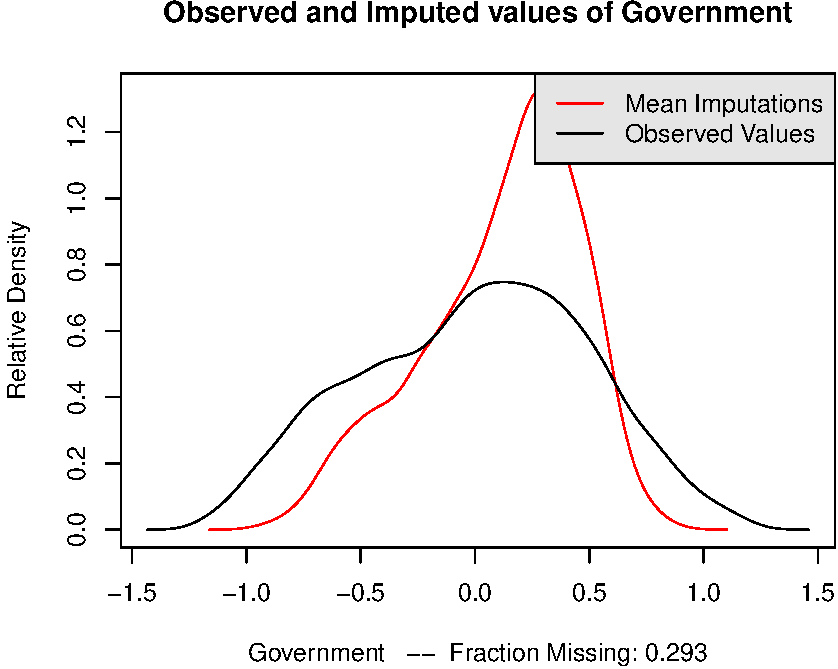
\includegraphics{figures/missing3-1.pdf}
\caption{Distributions Before and After Multiple Imputation (2)}
\end{figure}

\clearpage

\begin{figure}[htbp]
\centering
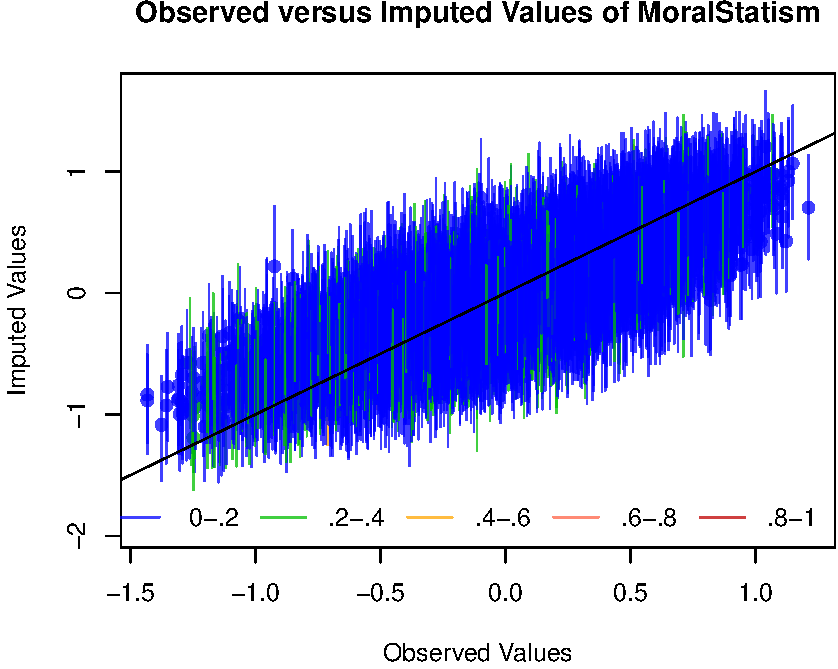
\includegraphics{figures/missing4-1.pdf}
\caption{Diagnostic Plot for Overimputation (1)}
\end{figure}

\begin{figure}[htbp]
\centering
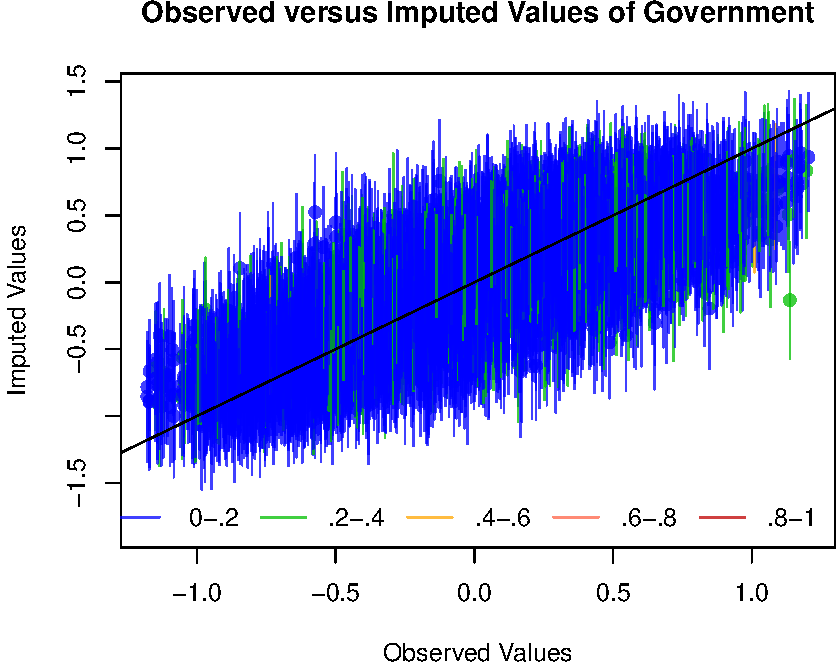
\includegraphics{figures/missing5-1.pdf}
\caption{Diagnostic Plot for Overimputation (2)}
\end{figure}

\clearpage

\begin{figure}[htbp]
\centering
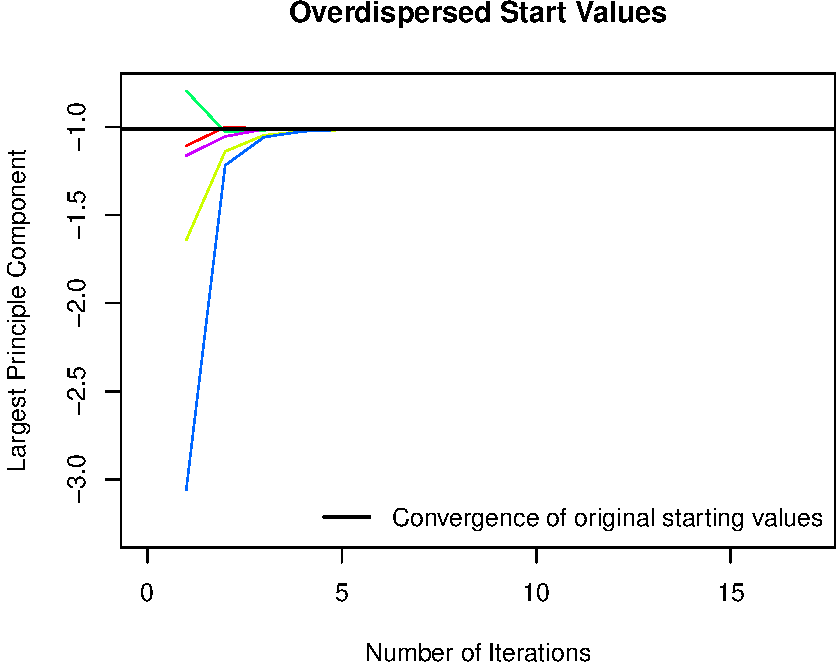
\includegraphics{figures/missing6-1.pdf}
\caption{Diagnostic Plot for Dispersion}
\end{figure}

\subsubsection{Matching and Sensitivity}\label{matching-and-sensitivity}

The algorithm obtains the matched pairs of those ``treated'' and not
treated to governmentalism and moral statism which are otherwise
optimally balanced in the propensity to be treated. The average
treatment effect for the treated obtained from this subset will
approximate that which we would obtain from a randomized experiment,
unless some unobserved factor shapes the propensity to be treated.
Although the possibility of omitted variables can never be ruled out, we
can quantify the sensitivity of these matching estimates to some
potential unobserved source of bias. Thus, we also report sensitivity
bounds as developed by Rosenbaum (1988), using the R package \emph{rbounds} (Keele 2014).

We generate matching estimates for the effect of governmentalism and the
interaction term, one at a time, using one-to-one genetic matching with
replacement (Sekhon 2011). We ignore moral statism because the main analyses suggest
it does not have an independent effect. In each case, ``treatment'' is
defined as having a value above the sample mean of the variable of
interest. For each estimate, we balance on all covariates in Model 2
except the two components of the interaction term and including the
treatment variable's propensity scores with respect to those covariates.
We do not balance on the components of the interaction term, or the
interaction term itself, because this would remove the covariation of
governmentalism and moral statism the effect of which we wish to test,
but we do include the components and the interaction term as covariates.

The average treatment effect on those ``treated'' with greater than the
mean level of governmentalism is -0.025, with a standard error of 0.012
(p=.04). The Rosenbaum bounds for this effect suggest that for it to
become statistically insignificant at the 95\% confidence level, the
odds of differential assignment to treatment due to an unobserved factor
would have to be about 1.45. The average treatment effect on those
``treated'' with greater than the mean level of the interaction term is
-0.022, with a standard error of 0.01 and a (p=.03). The Rosenbaum
bounds for this effect suggest that for it to become statistically
insignificant at the 95\% confidence level, the odds of differential
assignment to treatment due to an unobserved factor would have to be
about 1.39. The direction and statistical significance of the key
relationship in Model 2 (the interaction term), and one of its
independent components (governmentalism), do not appear to be spurious
artifacts of systematic assignment into treatment from any of the other
main covariates making individuals more likely to be misarchist.

\clearpage

\subsection{References}

Fabrigar, Leandre R, Duane T Wegener, Robert C MacCallum, and Erin J
Strahan. 1999. ``Evaluating the use of exploratory factor analysis in
psychological research.'' \emph{Psychological Methods} 4(3): 272--99.

Honaker, James, Gary King, and Matthew Blackwell. 2008. ``Amelia II: A
Program for Missing Data.'' \emph{Journal of Statistical Software}
45(i07).

Imai, Kosuke, Gary King, and Olivia Lau. 2009. ``Zelig: Everyone's
Statistical Software.'' \url{http://gking.harvard.edu/zelig}.

Keele, Luke J. 2014. ``rbounds: Perform Rosenbaum bounds sensitivity
tests for matched and unmatched data.''
\url{https://cran.r-project.org/web/packages/rbounds}.

Montgomery, Jacob M, and Brendan Nyhan. 2010. ``Bayesian Model
Averaging: Theoretical Developments and Practical Applications.''
\emph{Political Analysis} 18(2): 245--70.

Raftery, Adrian E., Jennifer Hoeting, Chris Volinksy, Ian Painter, and Ka Yee Yeung. 2015. ``BMA: Bayesian Model Averaging.''
\url{https://cran.r-project.org/web/packages/BMA/}.

Rosenbaum, Paul R. 1988. ``Sensitivity Analysis for Matching with
Multiple Controls.'' \emph{Biometrika} 75(3): 577--81.

Sekhon, Jasjeet S. 2011. ``Multivariate and Propensity Score Matching
Software with Automated Balance Optimization: The Matching Package for
R.'' \emph{Journal of Statistical Software} 42(7).


\end{document}